%preámbulo
\documentclass[12pt,oneside,FLEQN]{report}
\usepackage{amssymb,amsthm,amsmath,enumerate,graphicx,tabularx}
\usepackage[utf8]{inputenc}
\usepackage[hidelinks]{hyperref}
\usepackage[spanish]{babel}
\usepackage[rflt]{floatflt}
\usepackage{multicol}
\usepackage{tcolorbox, empheq}
\tcbuselibrary{skins,breakable,listings,theorems}
\usepackage{tikz,tkz-tab}
\usetikzlibrary{matrix,arrows, positioning,shadows,shadings,backgrounds,calc, shapes, tikzmark}
\usepackage{subfigure}
\usepackage{caption}
\usepackage[a4paper]{geometry}
\geometry{top=1.5cm, bottom=1.5cm, left=3cm, right=3cm}
\usepackage{ragged2e}
\newcommand{\marcar}[3]{\tikz[overlay,remember picture,baseline=-2pt] \node[circle,#1,draw,text=black, inner sep=1pt] (#2) { #3};}
\parindent=0cm
\usepackage{listings}
\hypersetup{
colorlinks=true,
linkcolor=black,
filecolor=magenta,
urlcolor=cyan,
citecolor=greenwhats
}
\usepackage[dvipsnames,table]{xcolor}
%\usepackage{lscape}
\usepackage{enumitem}
\definecolor{greenwhats}{RGB}{37, 211, 102}
\definecolor{gris}{rgb}{0.33, 0.41, 0.47}
\usepackage{fancyhdr}
\usepackage{natbib}
\usepackage{colortbl}
\usepackage{array,booktabs}
%\usepackage{pdflscape}
\usepackage{longtable}
\definecolor{codeturquoise}{RGB}{72,202,228}
\definecolor{codeyellow}{RGB}{255,170,51}
\definecolor{codepurple}{RGB}{255, 203, 242}
\definecolor{codegreen}{RGB}{149,213,178}
\definecolor{backcolour}{RGB}{73,80,87}
\definecolor{white}{RGB}{255,255,255}
\lstdefinestyle{estilochidori}{
backgroundcolor=\color{backcolour},
commentstyle=\color{codeyellow},
keywordstyle=\color{codeturquoise},
numberstyle=\tiny\color{codegreen},
stringstyle=\color{codepurple},
basicstyle=\ttfamily\footnotesize\color{white},
breakatwhitespace=false,
breaklines=true,
captionpos=b,
keepspaces=true,
numbers=left,
numbersep=5pt,
showspaces=false,
showstringspaces=false,
showtabs=false,
tabsize=2
}
\lstset{style=estilochidori}
\begin{document}
{
\fontfamily{qag}\selectfont
\begin{titlepage}
        \topmargin=0cm
        \centering

        {\bfseries\LARGE Universidad Autónoma de Querétaro \par}
        \vspace{1cm}
        {\scshape\Large  Facultad de Ingenier\'ia  \par}
        \vspace{2cm}
        \centering
        \begin{figure}[!h]
        \centering
                
\includegraphics[height=5cm]{Logouaq.png}
        \end{figure}
        \vspace{3cm}
        {\itshape\large Tarea 6: Descompocisión LU\par}
        \vspace{3cm}
        {\Huge Análisis numérico \par}
        \vspace{2cm}
        {\Large Autor: \par}
        {\large J.A. Salinas Sánchez \par}
        {\large Marzo2022 \par}
\end{titlepage}
\tableofcontents
\chapter{Introducción}
A pesar de ya conocer múltiples métodos, todos muy eficaces, universales y bastante precisos en cuanto a la resolución de sistemas de ecuaciones se refiere. Algunos de estos métodos pecan de poco eficientes según la cantidad de datos a tratar, del sistema en sí o solamente de su mero funcionamiento. Es por eso que hoy se explora la opción de utilizar el método de factorización LU o descomposición {\bf Lower-Upper} de sus siglas en inglés.\\

Como lo indica su nombre en inglés, la descomposición/factorización LUconsiste en buscar dos matrices triangulares, una superior ({\it Upper}) y una inferior ({\it Lower}), las cuales, al multiplicarse, regresen a la matriz original como resultado. El propósito de hacer esto es descomponer un sistema de ecuaciones nxn original en dos sistemas de ecuaciones más simples que pueden ser resuletos con cualquier otro método. Pudiendo reducir la magnitud del algoritmo desde $O(n^{3})$ hasta $O(n^{2})$.\\

Al igual que la factorización de expresiones algebraicas escalares o de cualquier otro objeto matemático, ésta se basa en el principio de hacer una ecuación entre cada uno de sus términos y un factor, de modo que cuando se multiplique a los términos por dicho factor, se obtenga de regreso la expresión original. Para ello, siguiendo las reglas de la multiplicación entre matrices, las matrices L y U tienen que ser cuadradas del mismo tamaño de la matriz original A, tienen que ser diagonales inferior y superior, respectivamente, y una tiene que tener una diagonal de sólo unos. Entonces, se buscaría lo siguiente:
\begin{align}
	A=L\cdot U=
	\begin{bmatrix}
		L_{11}&\hdots&L_{1n}\\
		\vdots&\hdots&\vdots\\
		L_{n1}&\hdots&L_{nn}\\
	\end{bmatrix}
	\cdot
	\begin{bmatrix}
		U_{11}&\hdots&U_{1n}\\
		\vdots&\hdots&\vdots\\
		U_{n1}&\hdots&U_{nn}\\
	\end{bmatrix}
	=\\
	\begin{bmatrix}
		A_{11}&\hdots&A_{1n}\\
		\vdots&\hdots&\vdots\\
		A_{n1}&\hdots&A_{nn}\\
	\end{bmatrix}\therefore \sum_{i,j=1}^{n}L_{ij}U_{ji}=A_{ij}
\end{align}
Lo curioso es que los coeficientes inferiores de la matriz L son los factores utilizados en la eliminación gaussiana, por lo que se puede aplicar eliminación gaussiana sobre A y guardar los coeficientes en L, resolver L y anexar los términos independientes en U, para luego resolver U. Aquí es donde se puede simplificar aún más el algoritmo.
\chapter{Metodología}
	Dependiendo del problema, se usó un script el cual incluía sólo la resolución mediante descomposición LU con o sin pivoteo, o que incluía lo anterior más la comprobación de la descomposición. Se muestra en el siguiente pseudocódigo.
		\lstinputlisting{pseudocodigo.txt}
\section{Problemas}
	\subsection{9.2}
		\lstinputlisting{LU2.py}
		\begin{figure}[!h]
			\centering
			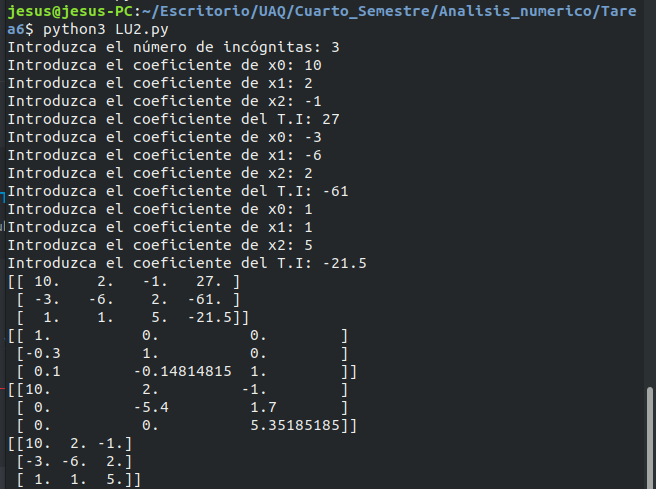
\includegraphics[scale=0.5]{102.png}
			\caption{Programa que muestra las matrices U y L en las cuales se descompuso la matriz de coeficientes del sistema de ecuaciones original, y cómo su multiplicación devuelve la matriz original.}
		\end{figure}
	\subsection{9.3}
		\lstinputlisting{LU.py}
		\begin{figure}[!h]
			\centering
			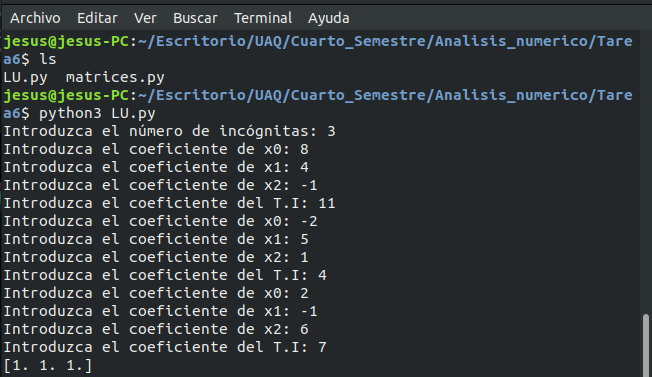
\includegraphics[scale=0.5]{103.png}
			\caption{Sistema de ecuaciones resuelto mediante descomposición LU.}
		\end{figure}
	\subsection{9.4}
		\lstinputlisting{LU.py}
		\begin{figure}[!h]
			\centering
			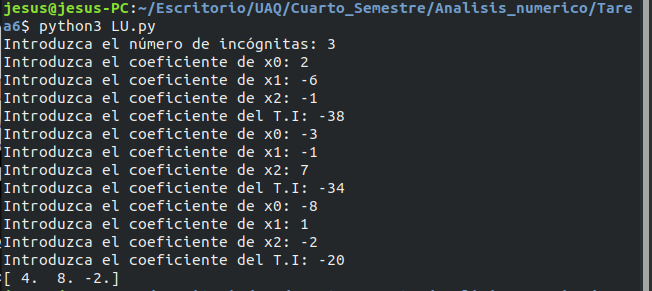
\includegraphics[scale=0.5]{104.png}
			\caption{Sistema de ecuaciones resulteo con factorización LU.}
		\end{figure}
	\subsection{9.7}
		\lstinputlisting{LU2.py}
		\begin{figure}[!h]
			\centering
			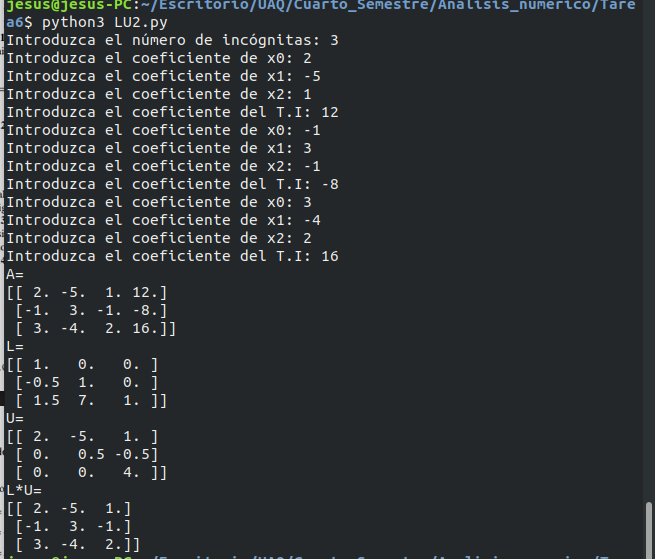
\includegraphics[scale=0.5]{107.png}
			\caption{Comprobación del éxito de una descomposición LU en el sistema mostrado.}
		\end{figure}
	\subsection{9.19}
\chapter{Conclusión}
A pesar de la ya existencia y conocimiento de distintos métodos de resolución de sistemas de ecuaciones lineales, es necesario, por la mejora considerable en eficiencia y por la flexibilidad para resolver más sistemas de ecuaciones. Además de aprovechar las propiedades algebraicas de los tensores de n dimensión, lo que después podría ayudar a desarrollar algoritmos para otras aplicaciones.
\begin{thebibliography}{1}
	\bibitem [1]{1} Chapra, S.C., 2015. In R. P. Canale, ed. Métodos numéricos para ingenieros. McGrawHIll Education, pp. 219–236. 
\end{thebibliography}
}
\end{document}
